\documentclass[12pt]{article}
\usepackage[utf8]{inputenc}
\usepackage{float}
\usepackage{amsmath}
\usepackage{tikz}
\usetikzlibrary{positioning}

\usepackage[hmargin=3cm,vmargin=6.0cm]{geometry}
%\topmargin=0cm
\topmargin=-2cm
\addtolength{\textheight}{6.5cm}
\addtolength{\textwidth}{2.0cm}
%\setlength{\leftmargin}{-5cm}
\setlength{\oddsidemargin}{0.0cm}
\setlength{\evensidemargin}{0.0cm}

\begin{document}

\section*{Student Information } 
%Write your full name and id number between the colon and newline
%Put one empty space character after colon and before newline
Full Name :  Hasan Küreli\\
Id Number :  2580751\\

% Write your answers below the section tags
\section*{Answer 1}
Let $G(x)$ be the generating function for the sequence $\{a_n\}$, that is, $G(x)= \sum_{n=0}^{\infty} a_n \cdot x^n $ \\
$x \cdot G(x) = \sum_{n=0}^{\infty} a_n \cdot x^{n+1} = \sum_{n=1}^{\infty} a_{n-1} \cdot x^n$\\
$x^2 \cdot G(x) = \sum_{n=0}^{\infty} a_n \cdot x^{n+2} = \sum_{n=2}^{\infty} a_{n-2} \cdot x^n$\\\\
$G(x) - 3 x\cdot G(x) - 4x^2 \cdot G(x) = \sum_{n=0}^{\infty} a_n \cdot x^{n} - 3\cdot \sum_{n=1}^{\infty} a_{n-1} \cdot x^{n} -4\cdot \sum_{n=2}^{\infty} a_{n-2} \cdot x^{n}$\\
$(1- 3x -4x^2)\cdot G(x) = a_0 + a_1 \cdot x -3 x \cdot a_0 + \sum_{n=2}^{\infty} (a_n - 3a_{n-1} - 4a_{n-2}) \cdot x^{n} $\\
By using the recurrence relation $a_n - 3a_{n-1} - 4a_{n-2} = 0$ and $a_0,a_1=1$:\\
$(1- 3x -4x^2)\cdot G(x) = 1 - 2x$\\
$G(x) = \frac{1-2x}{1- 3x -4x^2}$\\
By using partial fractions:\\
$G(x) = \frac{A}{1-4x} + \frac{B}{x+1}$\\
$A - 4B = -2$\\
$A+B = 1$\\
$A= 2/5$\\
$B=3/5$\\
$G(x) = \frac{2/5}{1-4x} + \frac{3/5}{1+x} $\\
Using the identity: 
$\frac{1}{1-ax} =\sum_{n=0}^{\infty} a^n \cdot x^n $\\
$G(x)= \frac{2}{5}\cdot \sum_{n=0}^{\infty} 4^n \cdot x^n + \frac{3}{5} \cdot \sum_{n=0}^{\infty} (-1)^n \cdot x^n$\\
So we have:\\
$$a_n = \frac{2}{5}\cdot 4^n + \frac{3}{5} \cdot (-1)^n$$

\section*{Answer 2}
\subsection*{a) }
Let's say that $f(x)$ is the generating function.\\
It's of the form:\\
$$f(x) = a_0x^0 + a_1x^1 + a_2x^2 + a_3x^3+...$$
For the given sequence:\\
$$f(x) = 2x^0 + 5x^1 + 11x^2 + 29x^3+...$$
We know that  $$\frac{2}{1-x} = 2 \cdot \sum_{n=0}^{\infty} x^n$$
So substracting $\frac{2}{1-x}$ we get:\\
$$f(x) - \frac{2}{1-x}= 0x^0 + 3x^1 + 9x^2 + 27x^3+...$$
$$f(x) - \frac{2}{1-x}+1= x^0 + 3x^1 + 9x^2 + 27x^3+...$$
$$f(x) - \frac{2}{1-x}+1= x^0 + 3^1x^1 + 3^2x^2 + 3^3x^3+...$$
Since $$x^0 + 3^1x^1 + 3^2x^2 + 3^3x^3+... = \sum_{n=0}^{\infty} 3^n \cdot x^n = \frac{1}{1-3x}$$
$$f(x) - \frac{2}{1-x}+1= \frac{1}{1-3x}$$
$$f(x) = \frac{1}{1-3x}+\frac{2}{1-x}-1 $$
$$f(x) = \frac{-3x^2 - 3x +2}{3x^2 - 4x +1} $$

\subsection*{b) }
By using partial fractions:\\
$$G(x) = \frac{7-9x}{1-3x+2x^2} = \frac{A}{2x-1}+\frac{B}{x-1}$$\\
$A + 2B = -9$\\
$-A - B = 7$\\
$A = -5 $\\
$ B = -2$\\
We know that  $$\frac{1}{1-ax} = \sum_{n=0}^{\infty}a^n \cdot x^n$$\\
$$G(x) = \frac{5}{1-2x}+\frac{2}{1-x} = 5\sum_{n=0}^{\infty} 2^n \cdot x^n + 2 \cdot\sum_{n=0}^{\infty} x^n $$\\
So we have:\\
$$a_n = 2 + 5\cdot 2^n$$
Thus, the sequence corresponding to the generating function:\\
$$< 7, 12, 22, 42, 82, 162, ... >$$\\


\section*{Answer 3}
\subsection*{a) }
Let's check if R is reflexive:\\
$aRa$ means $(a^2 +a^2 = n^2) \vee (a^2 + n^2 = a^2) $\\
For first condition since n and a are integers n can't be equal to $a\sqrt{2}$ which is not an integer.\\
For second condition for n to be an edge it must be a positive integer and can't be zero.\\
So it is not reflexive and hence, not an equivalence relation.

\subsection*{b) }
Because $2x_1 + y_1 = 2x_1 + y_1 $ for all real numbers $x_1,y_1$. Hence $(x_1,y_1)R(x_1,y_1)$  for all real numbers $x_1,y_1$. So R is reflexive.\\
Suppose $(x_1,y_1)R(x_2,y_2)$. Then $2x_1 + y_1 = 2x_2 + y_2 $, so $2x_2 + y_2 = 2x_1 + y_1 $ is also true. Hence $(x_2,y_2)R(x_1,y_1)$, it follows that R is symmetric.\\
If $(x_1,y_1)R(x_2,y_2)$ and $(x_2,y_2)R(x_3,y_3)$, $2x_1 + y_1 = 2x_2 + y_2 = 2x_3 + y_3$. Hence $(x_1,y_1)R(x_3,y_3)$. Thus, R is transitive.\\
Consequently $R$ is an equivalence relation.\\
Let's assume that $(x,y)$ is the equivalence class of $(1,-2)$.\\
So, $2x+y = 2\cdot1 - 2 = 0$.\\
$x= -\frac{y}{2}$\\
Let's say $y$ is equal to some constant $k$ then the equivalence class is of the form: $(-\frac{k}{2}, k)$\\
And it represents the line $y = -2x $ in the cartesian coordinate system.\\

\section*{Answer 4}
\subsection*{a) }
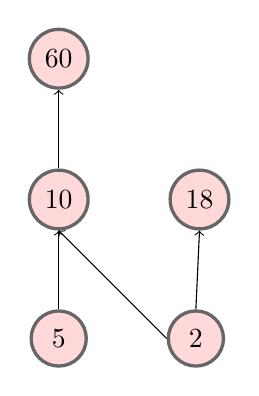
\begin{tikzpicture}[
roundnode/.style={circle, draw=black!60, fill=pink!60, very thick, minimum size=7mm},
]
%Nodes
\node[roundnode]      (maintopic)                              {10};
\node[roundnode]      (uppercircle)       [above=of maintopic] {60};
\node[roundnode]      (rightsquare)       [right=of maintopic] {18};
\node[roundnode]      (lowercircle)       [below=of maintopic] {5};
\node[roundnode]      (circle)       [right=of lowercircle] {2};

%Lines
\draw[->] (maintopic.north) -- (uppercircle.south) ;
\draw[->]  (lowercircle.north) --(maintopic.south);
\draw[->]  (circle.north) -- (rightsquare.south);
\draw[->] (circle.west)--(maintopic.south);

\end{tikzpicture}

\subsection*{b) }
Columns and rows are 2, 5, 10, 18, 60\\\\
$\begin{bmatrix}
1 & 0 & 1 & 1 & 1\\
0 & 1 & 1 & 0 & 1\\
0 & 0 & 1 & 0 & 1\\
0 & 0 & 0 & 1 & 0\\
0 & 0 & 0 & 0 & 1 
\end{bmatrix}$

\subsection*{c) }

$$(x,y)= \{ (10,2),(18,2), (60,2), (10,5), (60,5) , (60,10)\}$$\\
Columns and rows are 2, 5, 10, 18, 60\\\\
$\begin{bmatrix}
1 & 0 & 1 & 1 & 1\\
0 & 1 & 1 & 0 & 1\\
1 & 1 & 1 & 0 & 1\\
1 & 0 & 0 & 1 & 0\\
1 & 1 & 1 & 0 & 1
\end{bmatrix}$

\subsection*{d) }
If we are allowed to replace only a single element it is not possible because we must change either 2 or 5 and also remove 18 since its not related to anything but itself and this is not possible with a single change.\\
But if we are allowed to remove 2 and add 1 element. It is possible, for example we can remove 2 and 18 and add 1 instead we get:\\
$A= \{1,5,10,60\}$
And we would get a total ordering in this way.
 
\end{document}